The shared scorer uses the Qwen3.5-2B backbone and released Open-Jev LoRA parameters\supercite{openjev,lora}. Numerical observations enter learned encoders rather than being serialized as text. Sensor and thermal encoders each produce eight 128-dimensional embeddings; PLC and process context produce two and four. These 22 embeddings are projected to the backbone width, preceded by embedded task text, and followed by a learned summary embedding. The sequence is padded to 64 positions with an attention mask. The backbone output at the summary position is projected to a 256-dimensional state representation (Fig.~\ref{fig:architecture}).

One state encoding is shared across all nine candidates in a request. Each candidate's $20\times4$ held-command sequence and 32 physics features are encoded to 64 dimensions each. Their concatenation with the state representation forms a 384-dimensional input to a 128-unit hidden layer and scalar residual output. The released Open-Jev scalar head is replaced by these thermal modules. The backbone uses BF16 and the new head FP32, with no autoregressive text generation. LoRA rank, scale, and dropout are 8, 16, and zero.

\begin{figure*}[t]
\centering
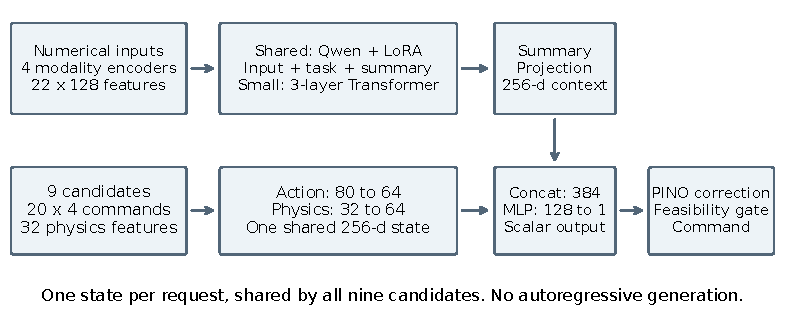
\includegraphics[width=\textwidth]{figures/residual_architecture.pdf}
\caption{Final residual-system computation. Both systems encode the numerical modalities and share one state representation across nine candidates. The shared system projects observation embeddings into the pretrained backbone; the small system uses a three-layer Transformer. The selected shared checkpoint retains the released backbone and LoRA parameters.}
\label{fig:architecture}
\end{figure*}

The compact scorer uses three Transformer layers of width 128, four attention heads, and feed-forward width 256, with the same context and candidate dimensions. Its full network is trainable during warmup. The final residual output layer is initialized to zero in both systems. The 32-component physics descriptor combines normalized absolute features with candidate-centered features scaled using training data. Candidate means are accumulated in FP64; two reserved calibration-feature entries are set to zero. All variants retain the separate PINO feasibility gate, including the variant with no physics input to the learned scorer.

